\chapter{Metodi e Algoritmi per la Compressione dell'Informazione}
Definito l'impianto teorico che governa la codifica di sorgente, passiamo ad analizzare i metodi con i quali si persegue l'obiettivo di rendere più efficiente la trasmissione e la memorizzazione dell'informazione.

Esistono due approcci distinti per affrontare il problema. Storicamente il primo è quello che si basa sulla \textbf{analisi statistica} delle informazioni per proporre una codifica più efficiente, il secondo invece evita l'approccio analitico a priori, appoggiandosi a un \textbf{dizionario} per abbassare la ridondanza dei dati. Non sono comunque approcci del tutto antitetici, in quanto spesso le codifiche di tipo \textit{statistico} possono risultare efficaci in combinazione con algoritmi a dizionario.

Altra differenza fondamentale tra i due approcci è il fatto che i metodi statistici operano sui singoli simboli, riducendo la \textit{ridondanza di codifica}, mentre quelli a dizionario manipolano sequenze ripetute di simboli, affrontando la \textit{ridondanza tra sequenze di simboli}. Questo comporta notevoli differenze nei risultati ottenibili in certe condizioni.

Esiste poi un terzo approccio, quello della trasformata Burrows-Wheeler, che senza un'analisi statistica, o conoscenza a priori, sfrutta le proprietà statistiche \textit{intrinseche} dei dati per realizzare un pre-processing dei dati in grado di favorire il lavoro degli algoritmi di compressione. 

\section{Metriche di Valutazione e Vincolo Lossless}
È fondamentale premettere che in questo capitolo tratteremo esclusivamente algoritmi di compressione \textbf{lossless} (senza perdita di informazione), in cui la sequenza decodificata risulta bit-a-bit identica a quella originale. 
Per valutare e confrontare le performance di questi algoritmi (indipendentemente dal loro approccio), si utilizzano metriche universali:
\begin{itemize}
    \item \textbf{Rapporto di Compressione (Compression Ratio - CR):} È il rapporto tra la dimensione dei dati originali e quella dei dati compressi ($CR = \frac{\text{Dim. Originale}}{\text{Dim. Compressa}}$). Un CR di 4 indica che i dati compressi occupano il 25\% dello spazio originale.
    \item \textbf{Risparmio di Spazio (Space Savings):} Misura la percentuale di spazio effettivamente risparmiata rispetto all'originale ($1 - \frac{1}{CR}$).
    \item \textbf{Bit rate medio:} Misurato in bit/simbolo, quantifica il numero medio di bit spesi per codificare un singolo carattere. Nei codici statistici, coincide con la lunghezza media $L_S(C)$.
\end{itemize}

\section{Algoritmi statistici}
Gli algoritmi statistici sono diretta conseguenza dell'introduzione del concetto di entropia e i successivi studi a riguardo.
Alla base del loro funzionamento c'è l'analisi delle frequenze di occorrenza dei singoli caratteri emessi dalla sorgente.

L'obiettivo matematico di questo approccio è minimizzare la lunghezza media del codice $L_S(C)$, abbattendo la \textit{ridondanza di codifica} per avvicinarsi il più possibile al limite teorico inferiore imposto dal Primo Teorema di Shannon (ovvero l'entropia $H(S)$ della sorgente).

Per raggiungere questo obiettivo si sfrutta un principio cardine tanto semplice quanto potente: 

\textbf{assegnare parole di codice (codeword) più corte ai simboli che compaiono con maggiore frequenza}, e codeword più lunghe a quelli più rari.

\paragraph{Fasi operative}
A livello implementativo, l'applicazione di un compressore statistico \textit{puro} richiede tipicamente due fasi distinte:
\begin{enumerate}
    \item \textbf{Costruzione del modello (Statistica):} Una prima scansione dei dati (o l'assunzione di un modello a priori) per calcolare la probabilità $p_i$ di ciascun simbolo dell'alfabeto.
    \item \textbf{Codifica:} La costruzione vera e propria dell'assegnamento (spesso rappresentata tramite un albero binario) e la successiva traduzione del flusso di simboli in una sequenza continua di bit.
\end{enumerate}

\subsection{Codifica di Shannon}
Per provare la validità del teorema della codifica di sorgente (\textit{Primo Teorema di Shannon}), Shannon ha ideato questa tecnica di compressione lossless per costruire codici prefissi. Sfrutta la conoscenza, stimata o misurata, dei simboli dell'alfabeto di sorgente.

Come vedremo, ci sono codifiche che risulteranno più efficienti, ma questa è stata la prima di questo tipo.

\begin{theorem}
Data $S$ sorgente senza memoria, se $\forall i \quad 1\leq  i \leq m$ si sceglie $l_i$ come l'\textbf{intero} \mbox{t.c.} $l_i = \lceil \log_d\frac{1}{p_i} \rceil$, allora si può trovare un codice prefisso $C$ \mbox{t.c.}
\[ \log_d\frac{1}{p_i} \leq l_i < \log_d \frac{1}{p_i} + 1\]
\[H_d(S) \leq L_S(C) < H_d(S) + 1\]

\begin{proof}
 La relazione $log_d\frac{1}{p_i} \leq l_i \leq \log_d \frac{1}{p_i} + 1$ vale solo se si possono trovare valori di $l_i$ che soddisfano la diseguaglianza di Kraft-McMillan.
 Sommando su tutti i valori di $i$ a destra e a sinistra, si ottiene la diseguaglianza di Kraft-McMillan.
 Notare che:
\begin{align*}
    \log_d\frac{1}{p_i} \leq l_i &\rightarrow -l_i \leq \log_d p_i \\
    &\rightarrow d^{-l_i} \leq p_i \\
    &\rightarrow \sum_{i=1}^m d^{-l_i} \leq 1
\end{align*}

Quindi tale codice può essere costruito.
Moltiplicando per $p_i$ la diseguaglianza $\log_d(\frac{1}{p_i}) \leq l_i < \log_d\frac{1}{p_i} +1$ e sommando per ogni $i$, si ottiene la tesi:
\[H(S) \leq L_S(C) \leq H(S) + 1\]
\end{proof}
\end{theorem}

\paragraph{\textbf{Non} ottimalità della codifica di Shannon}
Non è garantito che vengano generati dei codici compatti.
Ad esempio:

\begin{table}[htbp]
\centering
\renewcommand{\arraystretch}{1.5}
\begin{tabular}{
    >{\columncolor{blue!20}}c  % solo la prima colonna ha sfondo colorato
    | c 
    | c
}
\rowcolor{blue!50} 
%\textbf{S} & \textbf{Prob.} & \textbf{log(1/p\textsubscript{i})} \\
\textbf{S} & \textbf{Prob.} & \textbf{$\log(1/p_i)$} \\

\hline
$S_0$ & $\frac{2}{3}$ & $\log_2\left(\frac{3}{2}\right) \approx 0{.}58$ \\
$S_1$ & $\frac{2}{9}$ & $\log_2\left(\frac{9}{2}\right) \approx 2{.}17$ \\
$S_2$ & $\frac{1}{9}$ & $\log_2(9) \approx 3{.}17$ \\
\end{tabular}
\caption{Esempio non ottimale}

\end{table}

La codifica di Shannon propone lunghezze per le parole di codice $\{1,3,4\}$, ottenendo $L_S(C) = 1.78$.
Quindi $C$ \textbf{non} è compatto, perché ad esempio un codice $C'$ con lunghezze $\{1,2,2\}$ avrebbe $L_S(C')=1.33$. Ma essendo l'entropia pari a $H(S) \approxeq 1.22$, anche $C'$ non è ottimale.


\subsubsection{Estensione della sorgente}
Possiamo migliorare l'efficienza della codifica quando la semplice codifica simbolo per simbolo non dà buoni risultati?
Sì, possiamo farlo intervenendo sui simboli della sorgente.

Shannon dimostra che ci si può avvicinare all'entropia codificando non più i singoli simboli di $S$, ma blocchi di più simboli, ottenendo una nuova sorgente $S'$.\\
Si definisce $S'$ \textbf{estensione di ordine $n$} di una sorgente $S$, se i suoi simboli sono ottenuti raggruppando i simboli originari in sequenze di lunghezza $n$. Codificando $S'$ non si avrà perdita di informazione.
Codificando $S_n'$ con un codice\textbf{UD} istantaneo, questo soddisferà la seguente condizione:
\[H(S) \leq L_S(C) \leq H(S) + \frac{1}{n}\]
Se ne conclude che il meccanismo di estensione della sorgente consente, agendo sul valore di $n$, di avvicinarsi al \textit{limite di Shannon} quanto si desidera.
In particolare,
\[\lim_{n\to\infty} L_n = H(S)\]
\begin{osservazione}
In pratica aumentare $n$ per avvicinarsi all'entropia comporta un significativo aumento di complessità del decodificatore e inevitabilmente un ritardo di trasmissione.
\end{osservazione}

\paragraph{Generalizzazione}
Si dimostra che $H_d(S^n) = n \cdot H_d(S)$
Inoltre, $H_d(S^n)\leq L_{S^n}<H_d(S^n)+1$.
Considerando per ogni simbolo di $S$ la lunghezza media, si ottiene
\[H_d(S) = \frac{H_d(S^n)}{n}\leq \frac{L_{S^n}(C)}{n}<\frac{H_d(S^n)}{n}+\frac{1}{n} = H_d(S) + \frac{1}{n}\]
Con $L_n$ si indica la lunghezza media per i simboli di $S$, ovvero:
\[ L_n = \frac{L_{S^n}(C)}{n} \]
Quindi si realizza che  per blocchi sufficientemente grandi di simboli, si può raggiungere l'entropia
\[\lim_{n\to\infty}L_n = H_d(S)\]
\textbf{Problema:} il numero dei simboli della sorgente può crescere a dismisura. Scegliendo un valore per $n$ anche sufficientemente grande, non è comunque possibile sapere se e quanto si raggiunge il valore ottimale.

Serve quindi un modo per trovare codici compatti (\textbf{ottimali}) per la codifica delle sorgenti senza memoria.

\subsection{Codifica di Shannon-Fano (nel caso binario)}
Sviluppata indipendentemente da Claude Shannon e Robert Fano, questa tecnica rappresenta il primo approccio algoritmico pratico per la costruzione di un codice prefisso \textit{efficiente} basato sulle probabilità. La codifica di Shannon-Fano opera in modo costruttivo, adottando una strategia \textbf{top-down} (dall'alto verso il basso).

L'idea centrale è quella di dividere iterativamente l'alfabeto della sorgente, precedentemente ordinato in ordine di probabilità non crescente, in due sottoinsiemi con probabilità cumulativa il più possibile simile; ad ogni sottoinsieme/ramo  si assegna un bit distinto ($0$ o $1$). Questa procedura \textit{euristica} cerca di bilanciare l'albero di codifica in modo naturale secondo le probabilità dei simboli. Tuttavia, pur garantendo prestazioni notevoli, l'algoritmo si rivela \textbf{sub-ottimale}: non assicura matematicamente la minima lunghezza media possibile per la sorgente, difetto che verrà risolto in seguito dall'algoritmo di Huffman.

\textbf{Algoritmo:}
\begin{enumerate}[label=\arabic*., leftmargin=1.5em]
  \item Si elencano i simboli di $S$ in ordine di probabilità \textbf{non} crescente.
  \item Si divide la lista formando due gruppi di simboli tali che le somme di probabilità siano \textit{quasi} uguali.
  \item Si aggiunge una cifra $0$ a destra del primo gruppo, si aggiunge $1$ a destra di quelle del secondo gruppo.
  \item Ciascuno dei due gruppi è suddiviso con lo stesso criterio, appendendo i nuovi simboli alla codifica.
  \item Si continua fino a che ogni gruppo è costituito da un solo elemento.
\end{enumerate}

\begin{algorithm}
\caption{Costruzione Codice Shannon-Fano}
\begin{algorithmic}[1]
\Require Una lista di simboli $S$ con le loro probabilità $P$
\Ensure Un codice binario per ogni simbolo in $S$
\Statex
% Definiamo la funzione ricorsiva principale
\Function{ShannonFano}{Lista $L$}
    \If{$|L| > 1$} \Comment{Passo 5: Continua solo se il gruppo ha più di 1 elemento}
        \State Ordina $L$ in base alle probabilità in ordine \textbf{non} crescente \Comment{Passo 1}
        
        \State Dividi $L$ in due sottogruppi $L_1$ e $L_2$ 
        \Statex \hspace{\algorithmicindent} tali che $\sum_{s \in L_1} P(s) \approx \sum_{s \in L_2} P(s)$ \Comment{Passo 2}
        
        \For{ogni simbolo $s \in L_1$}
            \State $s\text{.codice} \leftarrow s\text{.codice} + \text{'0'}$ \Comment{Passo 3 (gruppo 0)}
        \EndFor
        
        \For{ogni simbolo $s \in L_2$}
            \State $s\text{.codice} \leftarrow s\text{.codice} + \text{'1'}$ \Comment{Passo 3 (gruppo 1)}
        \EndFor
        
        \State \Call{ShannonFano}{$L_1$} \Comment{Passo 4: Ricorsione sul primo gruppo}
        \State \Call{ShannonFano}{$L_2$} \Comment{Passo 4: Ricorsione sul secondo gruppo}
        
    \EndIf
    \State \Return \Comment{Se $|L| = 1$, la ricorsione per questo ramo termina}
\EndFunction
\Statex
\State Inizializza i codici di tutti i simboli $s \in S$ a stringa vuota
\State \Call{ShannonFano}{$S$} \Comment{Avvia la procedura sull'intera lista}
\end{algorithmic}
\end{algorithm}

\begin{table}[htbp]
\centering
\begin{tabular}{|c|c|c|c|c|c|c|c|c|}
\hline
\multirow{2}{*}{$x_i$} & \multirow{2}{*}{$P_i$} & \multicolumn{6}{c|}{Passi} & \multirow{2}{*}{Codeword} \\
\cline{3-8}
& & 1 & 2 & 3 & 4 & 5 & 6 & \\
\hline
$A$ & 0.50 & 0 & & & & & & 0 \\
\cline{3-5}
$B$ & 0.15 & 1 & 0 & 0 & & & & 100 \\
\cline{5-5}
$C$ & 0.15 & 1 & 0 & 1 & & & & 101 \\
\cline{4-5}
$D$ & 0.08 & 1 & 1 & 0 & & & & 110 \\
\cline{5-6}
$E$ & 0.08 & 1 & 1 & 1 & 0 & & & 1110 \\
\cline{6-7}
$F$ & 0.02 & 1 & 1 & 1 & 1 & 0 & & 11110 \\
\cline{7-8}
$G$ & 0.01 & 1 & 1 & 1 & 1 & 1 & 0 & 111110 \\
\cline{8-8}
$H$ & 0.01 & 1 & 1 & 1 & 1 & 1 & 1 & 111111 \\
\hline
\multicolumn{2}{|c|}{$H(X) = 2.15$} & \multicolumn{6}{c|}{} & $L = 2.18$ \\
\hline
\end{tabular}
\end{table}
\FloatBarrier

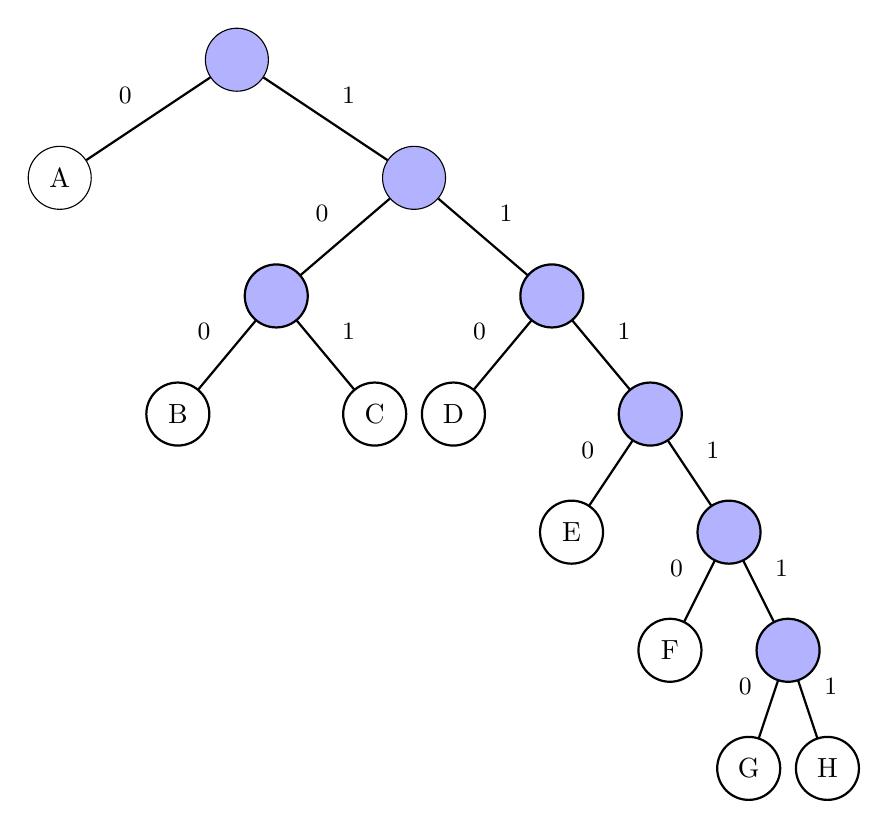
\begin{tikzpicture}[
    level distance=1.5cm,
    level 1/.style={sibling distance=4.5cm},
    level 2/.style={sibling distance=3.5cm},
    level 3/.style={sibling distance=2.5cm},
    level 4/.style={sibling distance=2cm},
    level 5/.style={sibling distance=1.5cm},
    level 6/.style={sibling distance=1cm},
    every node/.style={circle, fill=blue!30, draw, minimum size=8mm},
    leaf/.style={circle, fill=white, draw, minimum size=8mm, font=\normalsize},
    edge from parent/.style={draw, thick},
    edge label/.style={font=\small, fill=none, draw=none} % Rimosso 'auto'
]

\node {}
    child {
        node[leaf] {A}
        edge from parent node[above left, edge label] {0} % Modificato qui
    }
    child {
        node {} % Nodo P1
        child {
            node {} % Nodo P_BC, genitore diretto di B e C
            child {
                node[leaf] {B}
                edge from parent node[above left, edge label] {0} % Modificato qui
            }
            child {
                node[leaf] {C}
                edge from parent node[above right, edge label] {1} % Modificato qui
            }
            edge from parent node[above left, edge label] {0} % Modificato qui (arco da P1 a P_BC)
        }
        child {
            node {} % Nodo P_D, genitore di D
            child {
                node[leaf] {D}
                edge from parent node[above left, edge label] {0} % Modificato qui
            }
            child {
                node {} % Genitore di E
                child {
                    node[leaf] {E}
                    edge from parent node[above left, edge label] {0} % Modificato qui
                }
                child {
                    node {} % Genitore di F
                    child {
                        node[leaf] {F}
                        edge from parent node[above left, edge label] {0} % Modificato qui
                    }
                    child {
                        node {} % Genitore di G e H
                        child {
                            node[leaf] {G}
                            edge from parent node[above left, edge label] {0} % Modificato qui
                        }
                        child {
                            node[leaf] {H}
                            edge from parent node[above right, edge label] {1} % Modificato qui
                        }
                        edge from parent node[above right, edge label] {1} % Modificato qui
                    }
                    edge from parent node[above right, edge label] {1} % Modificato qui
                }
                edge from parent node[above right, edge label] {1} % Modificato qui
            }
            edge from parent node[above right, edge label] {1} % Modificato qui (arco da P1 a P_D)
        }
        edge from parent node[above right, edge label] {1} % Modificato qui (arco dalla Radice a P1)
    };

\end{tikzpicture}

\begin{table}[htbp]
    \centering
    \begin{tabular}{c c c c c}
        \toprule
        & $p_i$ & $\frac{1}{p_i}$ & $\log_2 \left(\frac{1}{p_i}\right)$ & $l_i\cdot p_i$ \\
        \midrule
        A & 0.50 & 2 & 1 & 0.50 \\
        B & 0.15 & 6.66 & 2.736964 & 0.45 \\
        C & 0.15 & 6.66 & 2.736964 & 0.45 \\
        D & 0.08 & 12.5 & 3.643856 & 0.24 \\
        E & 0.08 & 12.5 & 3.643856 & 0.32 \\
        F & 0.02 & 50 & 5.643856 & 0.10 \\
        G & 0.01 & 100 & 6.643856 & 0.06 \\
        H & 0.01 & 100 & 6.643856 & 0.06 \\
        \bottomrule
    \end{tabular}
\end{table}

Il valore dell'entropia è inferiore, ma la lunghezza media del codice è molto vicina al suo valore.

\subsubsection{Non ottimalità}
La codifica di Shannon-Fano non è ottimale; non è garantito che produca sempre la minima lunghezza media possibile per una data sorgente. In questo si differenzia dalla codifica di Huffman.

\textbf{Esempio:}

\begin{itemize}
    \item Con symbol rate $r=1000[\frac{simboli}{secondo}]$, la information rate sarebbe $R=r\cdot H(S) = 2150[\frac{bit}{secondo}]$.
    \item Un codice Shannon-Fano con $L_S=2.18$ richiede un bit rate $r_b= 2180 [\frac{bit}{sec}]$ (notare che $r_b > R$, come previsto per codici sub-ottimi).
    \item L'efficienza sarà:
    \[\eta = \frac{H(S)}{L_S} \cdot 100 = \frac{2.15}{2.18} \cdot 100 = 98.6\%\]
\end{itemize}

Un risultato comunque notevole, basti pensare che se si fosse utilizzata una codifica a lunghezza di parole fissa si sarebbe ottenuto un risultato decisamente peggiore:
\[r_b = L_S \cdot r = 3 \cdot 1000 = 3000\left[\frac{binit}{sec}\right]\]
\[\eta = \frac{H(S)}{L_S} \cdot 100 = \frac{2.15}{3} = 71.6\%\]

\subsection{Condizioni per ottimalità}
Si può dimostrare che, affinché un codice \textbf{\textit{UD} istantaneo} sia ottimo, si devono verificare queste condizioni:
\begin{enumerate}
    \item A simboli di $S$ meno probabili sono assegnate parole di codice più lunghe
    \[p_i > p_j \Rightarrow l_i \leq l_j\]
    \item Le due parole di codice meno probabili, quindi più lunghe, devono avere la stessa lunghezza
    \[l_{M-1} = l_M\]
    \item Delle parole di codice della stessa lunghezza, almeno due devono coincidere per tutti i bit tranne l'ultimo 
\end{enumerate}

\begin{proof}[Dimostrazione]
\begin{enumerate}
    \item Dato $C$ un codice \textbf{UD istantaneo ottimo} per cui non vale la condizione $1$, si costruisce $C'$ che differisce per la codifica di due parole che invalidano la condizione $1$. Di conseguenza $L_{C'} < L_C$; si ripete il procedimento fino a che la prima condizione è rispettata.
    \item Se $C$ è\textbf{UD}, nessuna parola è prefisso di un'altra. Se la $2$ non è rispettata, allora $l_M > l_{M-1}$; invertendo l'ultimo bit di $X_{M-1}$ il risultato è una parola non appartenente al codice e di lunghezza $l_{M-1}$ che può sostituire $l_{M}$.
    \item Si può accorciare di un bit la codifica di una parola se non vale la condizione $3$. 
\end{enumerate}
    
\end{proof}


\subsection{Codifica di Huffman}
La strategia di codifica proposta da David Huffman produce un codice ottimale dal punto di vista della lunghezza media, ovvero produce il minimo valore possibile per $L_S(C)$, approssimando il più possibile il limite imposto dal primo teorema di Shannon. Non produce necessariamente un codice assolutamente ottimo.

L'idea è nata grazie a un problema assegnato dal suo professore, Robert Fano, che chiedeva di trovare il codice binario più efficiente possibile.
All'idea già usata da Shannon e Fano di assegnare ai simboli della sorgente con minore frequenza parole di codice più lunghe, Huffman propose di usare un albero binario ordinato secondo le frequenze dei simboli.


L'algoritmo, con un approccio \textit{\textbf{bottom-up}}, produce un \textbf{albero binario completo} (\textit{albero di Huffman}) che identifica il codice. I codici di Huffman vengono usati in molte tecniche di compressione e, a seconda del tipo di input, consentono un risparmio tra il $20\%$ e il $90\%$.

\subsubsection{Codici prefissi ottimali}
Sia $C$ un codice \textbf{prefisso compatto} (o \textbf{ottimale}) per $S$ \mbox{t.c.} $c_i$ è la parola di codice associata al simbolo con probabilità $p_i$, e $p_1 \geq p_2 \geq \dots \geq p_m$
Allora:
\begin{enumerate}
    \item $p_j \geq p_k \to |c_k| \geq |c_j|$
    \item $|c_m| = |c_{m-1}|$ ovvero i simboli meno probabili hanno codeword della stessa lunghezza.
    
    Se $|c_m| > |c_{m-1}|$ basta rimuovere a $c_m$ l'ultimo simbolo, ottenendo un altro codice prefisso ma di lunghezza inferiore.
    \item \textbf{Almeno} due codewords tra quelle di lunghezza massima, differiscono \textbf{solo} per l'ultimo simbolo (bit).    
\end{enumerate}
Se tutte le parole di lunghezza massima $M$ differissero per un simbolo che non è l'ultimo, queste potrebbero essere sostituite dal prefisso di lunghezza $M-1$, e si avrebbe ancora un codice prefisso con una $L_S$ minore.

\subsubsection{Algoritmo di Huffman}
Sia data la sorgente $S = \begin{pmatrix}
s_1 & s_2 & \dots & s_m\\
p_1 & p_2 & \dots & p_m
\end{pmatrix}$ con le probabilità in ordine $p_1 \geq p_2 \geq \dots \geq p_m$
\begin{itemize}
    \item Si indica con $R(S)$ la \textbf{sorgente ridotta}, che si ottiene sostituendo i simboli meno probabili con un simbolo la cui proprietà è la somma della probabilità dei simboli che ha sostituito:
    \[
    R(S) = \begin{pmatrix}
s_1 & s_2 & \dots & (s_{m-1},s_m)\\
p_1 & p_2 & \dots & p_{m+1} + p_m
\end{pmatrix}
    \]
    \item Sia $C_R$ un codice prefisso per $R(S)$ e $z$ la parola di codice associata al simbolo $(s_{m-1},s_m)$. Il codice $C$ è ottenuto assegnando ad ogni parola della sorgente $S$ la stessa parola corrispondente per il simbolo di $R(S)$ e usando $z0$ per $c_m$ e $z1$ per $c_{m-1}$, è un codice prefisso.
    
    Inoltre, $L_S(C) = L_{R(S)}(C_R) + p_{m-1} + p_m$

    \item Se $C_R$ è ottimale, anche $C$ è ottimale.
    
    Se non fosse così dovrebbe esistere un codice prefisso ottimale (compatto) $C'$ per $S$ \mbox{t.c.}
    \[L_S(C') < L_S(C)\].
  
    Per la terza proprietà almeno due parole, $z_{m-1}$ e $z_m$, di codice di lunghezza massima devono differire solamente per l'ultimo simbolo.
    Consideriamo il codice $C'_R$ ricavato da $C'$ che associa al simbolo ($s_{m-1},s_m$) la parola di codice ottenuta rimuovendo da $z_m$ l'ultimo simbolo.
 
    Si ottiene così un codice \textbf{prefisso} \mbox{t.c.} $L_S(C') = L_{R(S)}(C'_R) + p_{m-1} + p_m$. 

    Quindi contro l'ipotesi di ottimalità di $C_R$, si avrebbe che $L_{R(S)}(C'_R) < L_{R(S)}(C_R)$.
\end{itemize}

Data una sorgente $S$, si produce una successione di sorgenti $S_i$ (con $i=0,\dots,m-2$) tale che:
\[
S_0 = S \text{ e } S_{i+1} = R(S_i)
\]
...
fino ad ottenere una sorgente con due soli simboli.

L'albero è così costruito \textit{bottom-up}, e ha i simboli della sorgente nelle foglie.

Le due foglie con probabilità più piccole diventano figli di uno stesso nodo avente come probabilità la somma di queste. Arrivati alla sorgente con due simboli si ottiene un codice compatto; proseguendo a ritroso si ricava un codice compatto per tutte le sorgenti, fino ad $S$.

Il codice di Huffman costruito in questo modo non è unico, ma qualunque codice di Huffman per una data sorgente è ottimale.

\paragraph{Esempio}

\paragraph{Costruzione del codice come albero}

\subsubsection{Algoritmo di compressione di Huffman con codici binari}
\begin{algorithm}
\caption{Costruzione Albero di Huffman}
\begin{algorithmic}[1]
\Require Testo in input $T$
\Ensure Radice dell'albero di Huffman

\State Calcola le occorrenze $\mathrm{occ}(a)$ per ogni simbolo $a \in T$
\State Inizializza una Coda a Priorità (min-heap) $Q$
\Statex 
\For{ogni simbolo $a$ con $\mathrm{occ}(a) > 0$}
    \State $n \gets \text{NuovoNodo}(\text{simbolo}=a, \text{prob}=\mathrm{occ}(a))$
    \State $Q.\text{Insert}(n)$
\EndFor
\Statex
\While{$Q.\text{size} > 1$}
    \State $nodoSinistro \gets Q.\text{ExtractMin}()$
    \State $nodoDestro \gets Q.\text{ExtractMin}()$
    \Statex
    \State $probSomma \gets nodoSinistro.\text{prob} + nodoDestro.\text{prob}$
    \State $nodoPadre \gets \text{NuovoNodo}(\text{prob}=probSomma)$
    \State $nodoPadre.\text{left} \gets nodoSinistro$
    \State $nodoPadre.\text{right} \gets nodoDestro$
    \Statex
    \State $Q.\text{Insert}(nodoPadre)$
\EndWhile
\Statex
\State \Return $Q.\text{ExtractMin}()$ \Comment{L'ultimo nodo rimasto è la radice}
\end{algorithmic}
\end{algorithm}


\begin{algorithm}
\caption*{\bluetext{Huffman}(A: array; n: intero)}
\begin{algorithmic}[1]
\State Q: Priority\_Queue;
\State 
\For{i = 1 \textbf{to} n}
    \State Insert(Q,A[i]) \hfill $\triangleright$ Con una \redtext{coda a priorità} basata su \redtext{lista}:
\EndFor
\State \hfill $\triangleright$ \bluetext{Primo ciclo:}
\State \hfill $\triangleright$ Esegue una operazione di 
\State \hfill $\triangleright$ accodamento per ognuna delle n
\State \hfill $\triangleright$ iterazioni - n O(1)
\State
\For{i = 1 \textbf{to} n - 1}
    \State \redtext{x} = Extract-Min(Q) \hfill $\triangleright$ \bluetext{Secondo ciclo:}
    \State \redtext{y} = Extract-Min(Q) \hfill $\triangleright$ Esegue due operazioni di estrazione
    \State "crea un nuovo albero con radice z e valore P$_x$ \hfill $\triangleright$ dalla coda e una di accodamento per
    \State + P$_y$ e con figli destro x e sinistro y" \hfill $\triangleright$ ognuna delle n-1 iterazioni - (n-1) O(n)
    \State Insert(Q,z) \hfill $\triangleright$ Totale: O(n$^2$)
\EndFor
\State
\State \textbf{return} Extract-Min(Q) \hfill $\triangleright$ Con una \redtext{coda a priorità} basata su \redtext{heap}:
\State \hfill $\triangleright$ Totale: O(n log n).
\State
\State \hfill $\triangleright$ \textit{Nota: l'algoritmo è un greedy}
\end{algorithmic}
\end{algorithm}

La coda di priorità può essere implementata tramite uno heap di alberi binari in cui la priorità è data dall'opposto della probabilità dei simboli.



\subsubsection{Limiti della codifica di Huffman}
La codifica richiede la conoscenza delle probabilità dei simboli della sorgente, e questo comporta un passaggio di preprocessing, e l'invio di questa informazione al codificatore. Quindi si ha un impatto sia sul tempo di codifica sia sulla dimensione dell'output.

\subsubsection{Decodifica di Huffman}
Il decodificatore deve basarsi sulle stesse informazioni sull'input usate per la codifica. Quindi l'intestazione del file compresso dovrà contenere o l'albero usato dal compressore, oppure le probabilità dei simboli della sorgente per poterlo ricostruire.

Ciò aumenta le dimensioni dell'output compresso e nel caso si debba ricostruire l'albero anche il tempo di decodifica.

\begin{algorithm}
\caption{Decodifica Huffman}
\begin{algorithmic}[1]
\State \textbf{Input:} Albero di Huffman, file compresso
\State \textbf{Output:} File di output decodificato
\Statex
\While{ci sono bit da leggere}
    \State Leggi un bit dal file compresso
    \State Usa il bit per attraversare l'albero di Huffman (0: sinistra, 1: destra)
    \If{nodo corrente è una foglia}
        \State Stampa il carattere ASCII corrispondente nel file di output
        \State Torna al nodo radice dell'albero di Huffman
    \EndIf
\EndWhile
\State Il programma termina quando non ci sono altri bit da decodificare 
\Statex \phantom{\textbf{Input:}}\hspace{\algorithmicindent} (o quando si raggiunge il numero di caratteri memorizzati nell'intestazione)
%\Statex \hspace{1.5em} (o quando si raggiunge il numero di caratteri memorizzati nell'intestazione)
\end{algorithmic}
\end{algorithm}

\subsubsection{Osservazioni sulla codifica Huffman}
L'algoritmo di Huffman rappresenta una soluzione ottima al problema della costruzione di codici prefissi a lunghezza variabile, minimizzando la lunghezza media del codice per una sorgente nota. Si può dimostrare che $L_S(C)$ rispetta il vincolo dettato dal teorema di Shannon, ovvero $L_S(C) \geq H(S)$.
In questo contesto si avvicina al limite teorico minimo, pur non raggiungendolo necessariamente, a causa del vincolo di impiegare lunghezze \textit{intere} per le codeword. 


Da notare che la costruzione dell'albero di Huffman \textbf{non} è univoca: in presenza di più coppie di simboli con probabilità minime uguali, le scelte sono tutte legittime. Si avranno codici differenti, tutti però ottimali.

In applicazioni pratiche, soprattutto in sistemi di comunicazioni con buffer a dimensione fissa, risulta vantaggioso impiegare codici con \textbf{varianza minima} nella lunghezza delle codeword, anche a scapito di un lieve aumento di $L_S(C)$. Lunghezze più omogenee facilitano la gestione del buffering e del padding dei dati.

Per ottenere codici a varianza minima, in fase di costruzione dell'albero a parità di probabilità, è sempre preferibile aggregare i nodi che rappresentano i sotto-alberi con altezza minore.

\paragraph{Ottimalità di Huffman}
La codifica \textit{per simbolo}, quando ad ogni simbolo corrisponde una codeword, risulta \textbf{ottimale} garantendo una \textbf{ridondanza minima}.

Per la ridondanza di codice definita da
\[\rho(C) = 1 - \eta(C)= \frac{L_S(C)-H_d(S)}{L_S(C)}\]
si trova un limite superiore alla ridondanza:
\[\rho_{Huff}(C) \leq p_1 + 1 - \log_2(e) + \log_2(\log_2(e)) \approx p_1 + 0.086\]
Con $p_1$ che indica la probabilità del simbolo più probabile.

La codifica sarà invece \textbf{assolutamente ottima}, eguagliando l'entropia della sorgente ($L_S(C) = H(S)$ con ridondanza nulla), se e solo se le probabilità sono potenze negative di due:
\[ L_S(C) = H(S) \iff \forall p_i \quad p_i = \frac{1}{2^{l_i}} \]

Si ottengono invece prestazioni \textit{sub ottimali} nel caso di sorgenti caratterizzate da \textit{molti} simboli ad \textit{altissima probabilità}. La necessità di assegnare ai simboli codifiche con un \textbf{numero intero} di caratteri limita la possibilità di rappresentare fedelmente le distribuzioni di probabilità rendendo più vantaggiosi, in certi casi, altre codifiche come la codifica aritmetica.

\paragraph{Estensione della sorgente per Huffman}
Da non confondere con il processo di aggregazione dei nodi dell'albero, l'estensione della sorgente interviene \textit{a priori} sui dati. Per superare il limite prestazionale imposto dai singoli simboli ad altissima probabilità, si raggruppano i simboli originali in blocchi di lunghezza $n$ (creando il super-alfabeto $S^n$) e solo successivamente si applica l'algoritmo di Huffman su di essi. In questo modo l'inefficienza dovuta al vincolo del bit intero viene frazionata su $n$ simboli, permettendo alla lunghezza media per simbolo originale di avvicinarsi all'entropia $H(S)$.


\subsection{Codifica Aritmetica}
La codifica aritmetica è una tecnica di compressione entropica, alternativa alla codifica di Huffman, ma basata su una strategia profondamente diversa. L'idea chiave, introdotta da Peter Elias, e formalizzata da Abramson nel 1963, consiste nel rappresentare un intero messaggio come un singolo numero reale compreso nell'intervallo $[0,1)$. 

Contrariamente a Huffman, dove ogni simbolo viene sostituito con una parola di codice, nella codifica aritmetica si lavora sul flusso completo dei simboli: l'intero messaggio determina progressivamente un intervallo sempre più ristretto in $[0,1)$. Il numero finale appartenente a tale intervallo è la rappresentazione codificata del messaggio.

In termini teorici, la lunghezza del codice prodotto tende a essere molto vicina all'entropia della sorgente, rendendo la codifica aritmetica quasi ottimale.


\subsubsection{Codifica aritmetica Vs Huffman}
In caso di distribuzioni di probabilità dei simboli asimmetriche, si avvicina maggiormente all'entropia rispetto alla codifica di Huffman.

Consideriamo una sorgente $S=\{a,b\}$ con $p(a)=\frac{99}{100}$ e $p(b)=\frac{1}{100}$; l'entropia sarà

\[H(S) = p(a)\log_2\left(\frac{100}{99}\right) + p(b)\log_2\left(\frac{100}{1}\right) \approx 0.08056\]
Qualunque codice prefisso, anche Huffman, impiega almeno un bit per simbolo, di conseguenza  $L_S$ deve essere almeno $1$, che in questo caso è molto maggiore del valore dell'entropia!

La codifica aritmetica aggira questo problema usando la codifica binaria di un numero frazionale

\paragraph{Esempio di codifica in binario}
Codifichiamo in binario $0.825$
\begin{align*}
0.825 \cdot 2 &= 1.65 &\quad U &= 1 \\
0.65 \cdot 2  &= 1.3  &\quad U &= 1 \\
0.3 \cdot 2   &= 0.6  &\quad U &= 0 \\
0.6 \cdot 2   &= 1.2  &\quad U &= 1 \\
0.2 \cdot 2   &= 0.4  &\quad U &= 0 \\
0.4 \cdot 2   &= 0.8  &\quad U &= 0 \\
0.8 \cdot 2   &= 1.6  &\quad U &= 1 \\
0.6 \cdot 2   &= 1.2  &\quad U &= 1
\end{align*}

Se durante la conversione binaria di un numero frazionario si verifica nuovamente un valore già incontrato nel processo iterativo, significa che la sequenza binaria sta entrando in un ciclo ripetitivo. In tal caso, si può interrompere l'algoritmo e rappresentare il numero come una frazione binaria periodica.

Ad esempio, la conversione di $0.825$ in binario genera la sequenza:

\begin{align*}
0.825 \times 2 = 1.65 & \quad \Rightarrow \quad 1 \\
0.65 \times 2 = 1.3  & \quad \Rightarrow \quad 1 \\
0.3 \times 2 = 0.6   & \quad \Rightarrow \quad 0 \\
0.6 \times 2 = 1.2   & \quad \Rightarrow \quad 1 \\
\text{e così via...}
\end{align*}


A un certo punto, il valore 0.6 si ripresenta, e quindi anche la sequenza di bit in uscita inizierà a ripetersi ciclicamente. Si ottiene dunque una rappresentazione periodica:
\[0.825 = 0.\overline{1101001}\]

\subsubsection{Algoritmo di Codifica Aritmetica}
\begin{algorithm}
\caption{Codifica aritmetica}
\begin{algorithmic}[1] % Il [1] numera le righe
    \Require Stringa da codificare $S$ su alfabeto $A$ con probabilità $P$
    \Ensure Lower bound dell'intervallo finale convertito in binario

    \State Inizializza l'intervallo a $[0, 1)$

    \For{ogni simbolo $s \in S$}
        \State Suddividi l'intervallo corrente in $n$ sotto intervalli, dove $n = |A|$
        \State Ogni sotto intervallo ha ampiezza proporzionale alla probabilità
        \State Seleziona il sotto intervallo corrispondente al simbolo $s$
        \State Aggiorna l'intervallo corrente a quello selezionato
    \EndFor

    \State \Return L'output è il lower bound dell'intervallo corrente...
\end{algorithmic}
\end{algorithm}



Per messaggi di lunghezza fissata $n$, gli intervalli generati non si sovrappongono mai. Conseguentemente, qualsiasi numero appartenente all'intervallo finale identifica in modo univoco il messaggio originale.
\paragraph{Esempio}
Si codifica la  stringa $BILL\space GATES$:

Per prima cosa servono le frequenze dei caratteri:
\begin{table}[htbp]
\centering
\begin{tabular}{|c|c|}
\hline
\textbf{Simbolo} & \textbf{Frequenza} \\
\hline
\texttt{(spazio)} & 0.1 \\
A & 0.1 \\
B & 0.1 \\
E & 0.1 \\
G & 0.1 \\
I & 0.1 \\
L & 0.2 \\
S & 0.1 \\
T & 0.1 \\
\hline
\end{tabular}
\caption{Distribuzione di frequenze dei simboli}
\end{table}

\begin{quote}
\textit{Nota: per spiegare l'algoritmo con l'esempio, i numeri che mostreremo saranno in base 10, ma ovviamente in realtà sono sempre in base 2.}
\end{quote}

\begin{table}[ht]
\centering
\begin{tabular}{|c|c|c|}
\hline
\textbf{Simbolo} & \textbf{Probabilità} & \textbf{Range} \\
\hline
spazio & 0.1 & [0.00, 0.10) \\
A      & 0.1 & [0.10, 0.20) \\
B      & 0.1 & [0.20, 0.30) \\
E      & 0.1 & [0.30, 0.40) \\
G      & 0.1 & [0.40, 0.50) \\
I      & 0.1 & [0.50, 0.60) \\
L      & 0.2 & \textbf{[0.60, 0.80)} \\
S      & 0.1 & [0.80, 0.90) \\
T      & 0.1 & [0.90, 1.00) \\
\hline
\end{tabular}
\caption{Distribuzione di probabilità e intervalli di codifica}
\end{table}


\begin{figure}[ht]
\centering
\begin{tikzpicture}[>=Stealth, node distance=1mm and 8mm, font=\small]
% Stack di sinistra
\foreach \i/\s in {8/spazio,7/A,6/B,5/E,4/G,3/I,2/L,1/S,0/T} {
    \node[draw, minimum width=1.2cm, minimum height=0.6cm] (L\i) at (0,0.6*\i) {\s};
}

% Stack di destra
\foreach \i/\s in {8/spazio,7/A,6/B,5/E,4/G,3/I,2/L} {
    \node[draw, minimum width=1.2cm, minimum height=0.6cm] (R\i) at (5,0.6*\i) {\s};
}

% Valori
\node at (0,-1) {0};
\node at (5,-1) {1};

% Frecce e valori intermedi
\draw[->, thick] (L6.east) -- ++(1,0) node[midway, above] {0.2} -- (R6.west);
\draw[->, thick] (L5.east) -- ++(1.3,0) node[midway, below] {0.3} -- (R4.west);

\end{tikzpicture}
\caption{Passaggio tra intervalli durante la codifica del simbolo B}
\end{figure}

Ricapitolando:
\begin{itemize}
    \item Dato un carattere $X$ con un \textit{intervallo iniziale}
    \[ [ \mathit{LowRange}(X), \mathit{HighRange}(X) ) \] 
    \item I nuovi limiti diventano
    \[\mathit{NewHigh}(X) \coloneq \mathit{OldLow} + (\mathit{OldHigh} - \mathit{OldLow}) \cdot \mathit{HighRange}(X)\]
    \[\mathit{NewLow}(X) \coloneq \mathit{OldLow} + (\mathit{OldHigh} - \mathit{OldLow}) \cdot \mathit{LowRange}(X)\]
    \item  Per codificare il simbolo $s$ (usando i numeri da $1$ a $n$) e il simbolo $i$ con probabilità $p_i$:
    \begin{itemize}
    \item $\mathit{low\_bound} = \sum_{i=1}^{s-1}p_i$
    \item $\mathit{high\_bound} = \sum_{i=1}^{s}p_i$
    \item $\mathit{range} = \mathit{high} - \mathit{low}$
    \item $\mathit{low} = \mathit{low} + \mathit{range} \cdot \mathit{low\_bound} $
    \item $\mathit{high} = \mathit{low} + \mathit{range} \cdot \mathit{high\_bound} $
    \end{itemize}
\end{itemize}

\paragraph{Decodifica}

La decodifica esegue lo stesso passaggio di restringimento dell'intervallo che avviene nella codifica:

\[\sum_{i=1}^{s-1}p_i \leq \frac{\text{value} - \text{low}}{\text{high} - \text{low}} \leq \sum_{i=1}^{s}p_i \]

\paragraph*{Algoritmo di decodifica}

\noindent
\textbf{INPUT:} Stringa da decodificare e alfabeto con distribuzione di probabilità

\begin{enumerate}
    \item Inizializza l'intervallo a $[0,1)$.
    \item Per ogni simbolo della stringa in input:
    \begin{enumerate}
        \item Suddividi l'intervallo corrente in sotto intervalli ($n=$ cardinalità dell'alfabeto). Ogni sotto intervallo avrà un'ampiezza proporzionale alla probabilità associata a ciascun elemento nell'alfabeto iniziale.
        \item Seleziona il simbolo corrispondente al sotto intervallo nel quale ricade il valore dell'input in analisi e seleziona tale intervallo come corrente.
    \end{enumerate}
\end{enumerate}

\vspace{1em}

\noindent
Si tratta di un algoritmo \textit{lossless} (senza perdita di informazione).

\paragraph{Gestione della terminazione}
Poiché la decodifica è un processo iterativo basato sul restringimento degli intervalli, l'algoritmo necessita di una condizione di arresto. Esistono due soluzioni pratiche:
\begin{enumerate}
    \item Trasmettere al decodificatore, come informazione accessoria (ad esempio nell'intestazione del file), la lunghezza esatta del messaggio originale.
    \item Introdurre nell'alfabeto di sorgente un simbolo speciale di fine file (\texttt{eof}) con una probabilità molto piccola (es. $p = 0.000001$). Quando il decodificatore incontra l'intervallo associato a \texttt{eof}, il processo termina.
\end{enumerate}

\paragraph{Perché funziona e perché è quasi ottimale}

La codifica aritmetica rappresenta un intero messaggio come un numero reale compreso in un intervallo, che viene progressivamente ristretto a ogni simbolo elaborato. A ciascun simbolo è associato un sotto intervallo proporzionale alla sua probabilità: i simboli più probabili riducono meno l'intervallo, mentre quelli meno probabili lo restringono di più.

L'ampiezza dell'intervallo finale dopo l'elaborazione dell'intera sequenza è pari al prodotto delle probabilità dei simboli che compongono il messaggio. Di conseguenza, il numero di bit necessari per rappresentare un numero all'interno di quell'intervallo è proporzionale a:

\[
-\log_2 \left( \prod_{i=1}^n p_i \right) = -\sum_{i=1}^n \log_2 p_i,
\]

cioè alla somma delle auto-informazioni dei simboli. Questo equivale all'informazione totale contenuta nel messaggio. In media, la lunghezza del codice per simbolo tende all'entropia della sorgente, rendendo la codifica aritmetica estremamente efficiente.

La codifica aritmetica è dunque \textit{quasi ottimale}: sebbene nella pratica siano necessari aggiustamenti dovuti alla rappresentazione finita (overflow, underflow, troncamento a interi), la lunghezza del codice si avvicina molto al limite teorico stabilito dall'entropia. Inoltre, può codificare simboli molto probabili in meno di un bit, cosa impossibile con codici prefisso come Huffman.



\section{Metodi basati su Dizionario}
Questa classe di metodi di compressione non sfrutta la conoscenza, o la stima, delle probabilità dei simboli della sorgente. Questo consente di affrontare situazioni per le quali la conoscenza statistica non è possibile o realizzabile, rendendo gli approcci visti finora inefficaci o improponibili.

I metodi \textit{statistici} operano sui singoli caratteri, e questo limita la compressione per il limite dato dall'entropia; i metodi a dizionario sostituiscono sequenze di simboli (\textit{frasi} o \textit{sottostringhe}) con riferimenti a un dizionario che ne memorizza i valori.

Questa tecnica, introdotta da Lempel e Ziv, costruisce in modo adattivo un dizionario, sopperendo alla conoscenza statistica a priori della sorgente. L'obiettivo è codificare pattern ricorrenti in modo efficiente. In questo modo risulteranno spesso più efficaci per dati in ingresso con molte ridondanze.

\subsection{Dizionario}
Formalizziamo un \textbf{dizionario} per un testo $T$ come un insieme 
\[D = \{(f,c) \mid f \in F, c \in C\}\]
dove
\begin{itemize}
    \item $F$ è un sottoinsieme di fattori (sottostringhe) del testo $T$
    \item $C$ è l'insieme delle corrispondenti parole di codice
\end{itemize}

\subsection{Dizionari statici}
Il modo più semplice di costruire un dizionario è una costruzione \textit{statica}, vale a dire si realizza il dizionario prima dell'effettiva compressione del dato.
Una delle forme più comuni di dizionario statico è la \textbf{codifica a digrammi}.
Il dizionario è costituito da tutte le lettere (simboli) della sorgente, e dall'aggiunta di \textbf{alcune} coppie di lettere, i digrammi.

Un esempio può essere un dizionario con i caratteri ASCII a 8 bit e 256 digrammi costituiti dalle coppie di caratteri più comuni.
\paragraph{Esempio}
Supponiamo che l'alfabeto sia $A=\{a,b,c,d,r\}$ e il dizionario sia il seguente
\begin{table}[ht]
\centering
\begin{tabular}{|c c|c c|}
\hline
\textbf{Codice} & \textbf{Frase} & \textbf{Codice} & \textbf{Frase} \\
\hline
000 & $a$ & 100 & $r$ \\
001 & $b$ & 101 & $ab$ \\
010 & $c$ & 110 & $ac$ \\
011 & $d$ & 111 & $ad$ \\
\hline
\end{tabular}
\caption{Dizionario per $A$}
\end{table}
Il codificatore analizza \textbf{due simboli per volta} e cerca corrispondenze nel dizionario.
\begin{itemize}
    \item Digramma identificato
        \begin{itemize}
            \item[$\Rightarrow$] digramma codificato
        \end{itemize}
    \item Digramma non identificato
        \begin{itemize}
            \item[$\Rightarrow$] codifica del primo carattere della coppia
        \end{itemize}
\end{itemize}
Nel nostro esempio, $abracadabra$ viene codificato con \texttt{101\,100\,110\,111\,101\,100\,000}.

Alternativamente ai digrammi, si potrebbero inserire nel dizionario frasi \textit{più lunghe}, sfruttando la conoscenza di parole comuni, come articoli o preposizioni, o parole ricorrenti. Si può sviluppare ancora di più questa tecnica sfruttando la conoscenza del tipo di messaggio, ad esempio se si tratta di un testo di argomento sportivo, o economico, etc. Quello che si può guadagnare in efficienza si perde in mancanza di flessibilità.

In conclusione i dizionari statici presentano notevoli limitazioni.

\subsection{Dizionari dinamici}
I metodi a dizionario rappresentano una evoluzione concettuale rispetto agli approcci statistici, abbandonando la necessità di una conoscenza a priori delle caratteristiche (probabilistiche) dell'input. I compressori ideati da Lempel e Ziv costruiscono il dizionario in modo \textbf{adattivo}, analizzando i dati durante la compressione stessa. Il principio fondante è che i dati già processati costituiscono il miglior dizionario possibile per codificare la parte successiva, sfruttando la ridondanza locale e le ripetizioni presenti nel flusso in ingresso.

L'approccio \textbf{adattivo} elimina due limiti dei dizionari statici:
\begin{enumerate}
    \item codebook generato implicitamente dall'input senza overhead di trasmissione del dizionario stesso.
    \item non si deve scegliere tra un dizionario \textit{troppo generico}, e quindi meno efficiente, e un dizionario \textit{troppo specifico} che sarebbe ottimale per un determinato tipo di dati, ma deficitario per altri tipi di dato.    
\end{enumerate}
Il meccanismo chiave si basa sulla \textbf{codifica per sostituzione}, le sottostringhe ricorrenti vengono sostituite con riferimenti a occorrenze precedenti, unite a porzioni di \textit{testo} non facenti parte di codeword. Questo dualismo permette al compressore di adattarsi a pattern non stazionari, superando i limiti dei codici fissi.

Gli algoritmi introdotti nel 1977 e nel 1978 da Lempel e Ziv sono \textbf{\textit{lossless}} e usati per la compressione di dati eterogenei. 

\subsubsection{LZ77}
L'idea chiave dei codificatori basati su dizionario, come LZ77, risiede nello sfruttare una caratteristica del dato da comprimere: la porzione precedentemente elaborata costituisce un ottimo dizionario \textit{intrinseco}, poiché, prendendo a riferimento un testo in linguaggio naturale, tipicamente condivide il medesimo linguaggio e la medesima struttura statistica del testo ancora da comprimere.

In questo modo il dizionario viene creato \textit{in divenire} dall'algoritmo e viene quindi meno la necessità di trasmettere il dizionario insieme ai dati compressi. Il decodificatore sarà in grado di ricostruirlo in modo adattivo e autonomo compiendo le stesse operazioni del codificatore.

Questo principio di \textbf{\textit{località}} si rivela valido non solo per testi, ma \textit{quasi} per ogni tipo di dato che vogliamo comprimere.


\paragraph{Codifica}
Il processo di codifica risulta semplice da implementare; i passi di codifica producono delle \textit{triple}:
\begin{enumerate}
    \item Offset: puntatore che indica quanto \textit{guardare indietro} nel testo precedentemente decodificato.
    \item Lunghezza della frase
    \item Carattere attualmente elaborato
\end{enumerate}
Ad esempio con un alfabeto $A = \{a,b\}$, il testo $abaaabaabb$ darebbe come risultato
\[\langle 0,0,a \rangle \quad \langle 0,0,b \rangle \quad \langle 2,1,a \rangle \quad \langle 3,2,b \rangle \quad \langle 5,3,b \rangle\]

\[
\underbrace{\langle 0,0,a \rangle}_{\text{a}} \quad
\underbrace{\langle 0,0,b \rangle}_{\text{b}} \quad
\underbrace{\langle 2,1,a \rangle}_{\text{aa}} \quad
\underbrace{\langle 3,2,b \rangle}_{\text{bab}} \quad
\underbrace{\langle 5,3,b \rangle}_{\text{aabb}}
\]
Il codificatore utilizza una \textbf{finestra scorrevole} sui dati in ingresso, divisa in due parti
\begin{itemize}
    \item \textbf{search buffer}: contiene la sezione già codificata
    \item \textbf{look-ahead buffer}: contiene i dati ancora da codificare
\end{itemize}
Ciò che separa i due buffer è il puntatore $i$, che indica l'inizio del look-ahead buffer.
Un ulteriore puntatore $j$ scorre il search-buffer a ritroso, partendo da $i$, cercando la più lunga sequenza possibile che sia un prefisso per il look-ahead buffer.

%\Large % Opzionale, per rendere il font più grande
\[
\underbrace{
    % --- Search Buffer ---
    % 1. "abbacc" in rosso
    \text{\textcolor{red}{\texttt{abbacc}}}
    % 2. "bbca" in rosso su sfondo giallo, con il puntatore 'j'
    \text{\colorbox{yellow}{%
        % Il puntatore 'j' è posizionato sopra la prima 'b'
        $\overset{
            \substack{
                \leftarrow j \\ \downarrow
            }
        }{
            % La base del puntatore ('b') è testo rosso
            \text{\textcolor{red}{\texttt{b}}}
        }$%
        % Il resto di "bbca" è anch'esso testo rosso
        \textcolor{red}{\texttt{bca}}%
    }}
    % 3. "bc" in rosso
    \text{\textcolor{red}{\texttt{bc}}}
}_{\text{search buffer}}
\underbrace{
    % --- Look-ahead Buffer (MODIFICATO) ---
    % 1. Spazio
    \text{\texttt{\ }}
    % 2. Il puntatore 'i' è posizionato sopra la prima 'b' in grassetto
    \overset{  % <--- ERRORE CORRETTO (rimosso $)
        \substack{
            i \\ \downarrow
        }
    }{
        % La base del puntatore ('b') è testo in grassetto
        \text{\texttt{\textbf{b}}}
    }%         % <--- ERRORE CORRETTO (rimosso $)
    % 3. Il resto di "bbca" è in grassetto
    \text{\texttt{\textbf{bca}}}
    % 4. La 'c' con la parentesi graffa sopra e il resto della stringa
    \overbrace{\text{\texttt{c}}} \text{\texttt{bcaacbbcb}}
}_{\text{look-ahead buffer}}
\]

L'output compresso consisterà in una sequenza di triple $\langle o,l,s \rangle$:
\begin{itemize}
    \item $o$, intero che rappresenta la distanza tra $i$ e $j$ (\textbf{offset})
    \item $l$, intero che rappresenta la lunghezza del prefisso individuato (\textbf{frase})
    \item $s$ carattere, il primo simbolo presente nel look-ahead buffer immediatamente successivo al prefisso, cioè codeword già presente nel dizionario
\end{itemize}

Nella codifica ad ogni passo si possono incontrare tre casistiche:
\begin{enumerate}
    \item Non si trova \textbf{alcun match} considerando il prossimo carattere da codificare
    \item \textbf{Match}
    \item \textbf{Match} che si estende \textit{dentro} il look-ahead buffer
\end{enumerate}

\begin{center}
% Correzione 2: Ridimensiona il diagramma per adattarlo alla larghezza della pagina
\resizebox{\textwidth}{!}{%
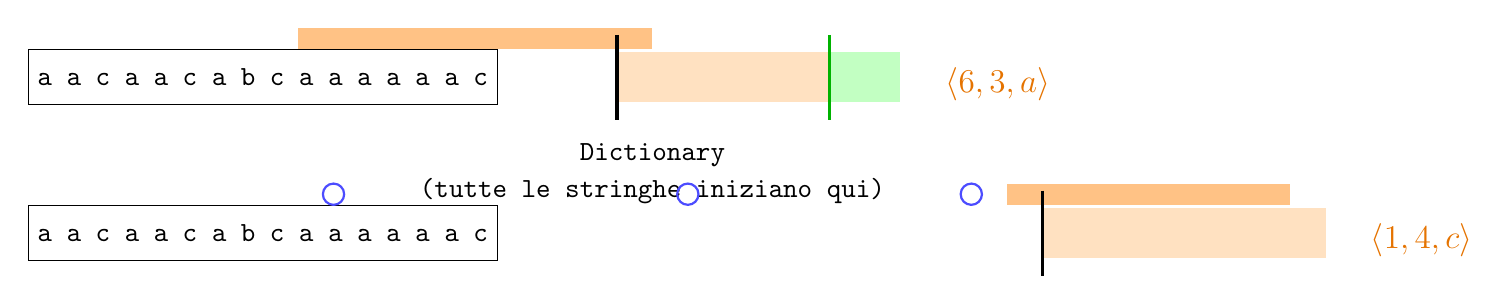
\begin{tikzpicture}[every node/.style={font=\ttfamily}, scale=0.9]

% Correzione 1: Rinominato \text in \diagramtext per evitare conflitti
\def\diagramtext{a a c a a c a b c a a a a a a c}
\def\startx{0}
\def\ytext{0}
\def\ystack{-2.2}

% Mostra la prima riga (testo completo)
% Correzione 1: Usa la macro \diagramtext
\foreach [count=\i] \char in \diagramtext {
    \node[draw, minimum size=0.7cm] at (\startx + \i, \ytext) {\char};
}

% Finestra di ricerca
\fill[orange!80, opacity=0.6] (\startx + 1.5, \ytext + 0.4) rectangle ++(5,0.3);

% Match trovato nella finestra
\fill[orange!30, opacity=0.8] (\startx + 6, \ytext - 0.35) rectangle ++(3,0.7);

% Match corrente nel lookahead buffer
\fill[green!40, opacity=0.6] (\startx + 9, \ytext - 0.35) rectangle ++(1,0.7);

% Linea divisoria tra finestra e buffer
\draw[very thick] (\startx + 6, \ytext + 0.6) -- ++(0,-1.2);

% Linea verde alla fine del match
\draw[very thick, green!70!black] (\startx + 9, \ytext + 0.6) -- ++(0,-1.2);

% Output tripla
\node[anchor=west, text=orange!90!black, font=\large\bfseries] at (\startx + 10.5, \ytext - 0.1) {$\langle 6,3,a\rangle$};

% Etichetta "Dictionary"
\node at (\startx + 6.5, \ytext - 1.1) {\bfseries Dictionary};
\node at (\startx + 6.5, \ytext - 1.6) {(tutte le stringhe iniziano qui)};

% Riga sottostante
% Correzione 1: Usa la macro \diagramtext
\foreach [count=\i] \char in \diagramtext {
    \node[draw, minimum size=0.7cm] at (\startx + \i, \ystack) {\char};
}

% Cerchi blu
\foreach \i in {2, 7, 11} {
    \draw[blue!70, thick] (\startx + \i, \ystack + 0.55) circle (0.15);
}

% Secondo match in basso
\fill[orange!80, opacity=0.6] (\startx + 11.5, \ystack + 0.4) rectangle ++(4,0.3);
\fill[orange!30, opacity=0.8] (\startx + 12, \ystack - 0.35) rectangle ++(4,0.7);

% Linea di separazione
\draw[very thick] (\startx + 12, \ystack + 0.6) -- ++(0,-1.2);

% Output secondario
\node[anchor=west, text=orange!90!black, font=\large\bfseries] at (\startx + 16.5, \ystack - 0.1) {$\langle 1,4,c\rangle$};

\end{tikzpicture}
} % Chiusura del \resizebox
\end{center}

In prima sintesi i passi dell'algoritmo sono:
\begin{enumerate}
    \item Cerca la copia più lunga che inizia prima
    \item Output della tripla $\langle \mathit{offset}, \mathit{length}, \mathit{symbol} \rangle$
    \item Aggiorna il cursore di $\mathit{length} + 1$
\end{enumerate}

%TODO: tabella processo di codifica

\paragraph{Copia simbolo per simbolo (Match estesi)}
Un dettaglio fondamentale di LZ77 è che la ricostruzione del prefisso non avviene \textit{in blocco}, ma rigorosamente \textbf{simbolo per simbolo}. 
Questa particolarità implementativa permette di gestire il caso in cui la lunghezza del match sia superiore all'offset ($l > o$), ovvero quando la ripetizione si estende oltre il search buffer e \textit{invade} il look-ahead buffer. 

%TODO: migliorare schema seguente
\begin{center}
\resizebox{\textwidth}{!}{%
  % Usiamo $...$ ma con \displaystyle per mantenere la grandezza
  $\displaystyle
  \textcolor{red}{\overbrace{aab??}} \to
  \textcolor{red}{\overbrace{{\underbrace{a}ab}\textcolor{black}{a}\textcolor{red}{?}}} \to
  \textcolor{red}{\overbrace{aab\textcolor{black}{aa}}} \to
  \textcolor{red}{\overbrace{aab\textcolor{black}{aa}}}b\to
  \textcolor{red}{\overbrace{aab\textcolor{black}{aa}}}ba \to
  \textcolor{red}{\overbrace{aab\textcolor{black}{aa}}baa}
  $
}
\end{center}

In questo scenario, quindi, un singolo offset (inferiore alla lunghezza del prefisso stesso) è sufficiente per istruire il decodificatore a generare un'intera sequenza ciclica continua.



\paragraph{Parametri \textit{strutturali} dell'algoritmo}
Come è necessario dimensionare il search buffer? Può essere \textit{infinito}?
No, non si permette all'algoritmo di cercare all'indietro indefinitamente fino all'inizio del flusso di dati.
Tipicamente il puntatore della finestra è di $12\text{ bit}$. Valori maggiori non offrono vantaggi, per il principio di località dei dati.

Per quanto riguarda la dimensione delle parole riferite, tipicamente non si va oltre i $4\text{ bit}$.

Usare indici e lunghezze maggiori permetterebbe di ottenere un numero minore di triple ma queste occuperebbero più spazio, e con una finestra di ricerca più grande inevitabilmente si impiegherebbe più tempo nella ricerca dei prefissi, è necessario un compromesso.

\paragraph{Capacità di compressione}
Nel caso in cui si comprima un file di testo (con caratteri a $8 \text{ bit}$), ogni tripla generata richiederà uno spazio di memoria pari a:
\[ n + m + 8 \text{ bit} \]
dove $n$ sono i bit necessari per l'indice (offset) e $m$ i bit per la lunghezza della frase.
Il numero di bit totali del file compresso sarà quindi la somma dei bit di tutte le triple: $(n + m + 8) \times \text{numero\_triple}$.
Il parametro di valutazione delle prestazioni è il \textbf{fattore di compressione}, definito come:
\[ \text{Fattore di compressione} = \frac{\text{Numero bit iniziali}}{\text{Numero bit finali}} \]

\paragraph{Codifica}

% Comandi personalizzati per la colorazione
\newcommand{\triple}[1]{\textcolor{blue}{#1}}
\newcommand{\lb}{\textcolor{red}{\{}}
\newcommand{\rb}{\textcolor{red}{\}}}
\begin{lstlisting}
Codifica LZ77
p = 1
WHILE (p < |S|) {
    Cerca il match massimo per S[p...] in S[p - n, ..., p-1]
// Supponi che il match sia in posizione p-i, con lunghezza l
    output della tripla <p-i, l, S[p+l]>
}
\end{lstlisting}



\paragraph{Decodifica}
\begin{lstlisting}
Decodifica LZ77
p = 1
FOREACH triple <f, l, c> {
    S[p ... p + l - 1] = S[p - f ... p - f + l - 1]
    // Supponi che il match occorre alla posizione p - f con lunghezza l
    S[p + l] = c
    p = p + l + 1
}
\end{lstlisting}


\paragraph{Prestazioni, limiti e vantaggi}
La decodifica è molto veloce, più della codifica che deve accollarsi la ricerca dei prefissi. Come già detto, accade che più il buffer è esteso, più le codewords possono essere lunghe e quindi essere in numero minore nell'output compresso. Parimenti le triple generate occuperanno più spazio e si spenderà più tempo cercando frasi in una finestra di dimensioni maggiori.

\paragraph{Varianti}
L'algoritmo LZ77 è stato oggetto di numerosi studi che hanno portato a diverse varianti, pur mantenendo l'idea generale di Lempel e Ziv. La più celebre è la variante \textbf{LZss} (Storer-Szymanski), che mira a eliminare lo spreco di bit dovuto all'obbligo di emettere sempre una tripla fissa.

Alcune modifiche all'implementazione delle triple:
\begin{description}[font=\normalfont]
    \item[Indice:] codifica variabile (Huffman) per rappresentarne il valore. Utile perché saranno molto più comuni offset \textit{piccoli}, per via del principio di località, e quindi si utilizzano meno bit per memorizzarli.
    
    \item[Lunghezza:] lo stesso vale per le lunghezze delle codewords, le lunghezze brevi sono più probabili e quindi si codificano con Huffman.
    
    \item[Simbolo (LZss):] il carattere in chiaro viene aggiunto solo quando serve (quando non c'è match). Si utilizza un \textbf{flag} di 1 bit per segnalare se i dati successivi rappresentano una coppia $\langle \text{offset}, \text{lunghezza} \rangle$ (riferimento al dizionario) oppure un singolo carattere non compresso.
\end{description}


\paragraph{Esempio di codifica e decodifica}
%TODO: esempio di codifica e decodifica

\subsubsection{LZ78}
L'algoritmo LZ78 si differenzia dal predecessore per alcune scelte implementative, ma sfrutta le stesse idee di base.
La prima differenza consiste nel limitare il numero di frasi, tra tutte quelle possibili, che possono andare a comporre il dizionario.

La prima differenza consiste nel limitare il numero di frasi, tra tutte quelle possibili, che possono andare a comporre il dizionario. Questo limite è teoricamente e praticamente necessario: sia per contenere l'occupazione di memoria, sia per mantenere fissa e ridotta la dimensione in bit dell'indice $i$ trasmesso in output (se il dizionario crescesse all'infinito, gli indici richiederebbero troppi bit, vanificando la compressione). Nello specifico viene utilizzato un \textit{trie} per memorizzare il dizionario e si vuole impedire che le dimensioni di quest'ultimo diventino eccessive.

Altra differenza sostanziale, legata a doppio filo con la precedente, è il non avere una finestra (o quantomeno un limite meno stringente) che limiti quanto a ritroso si possono cercare e riferire sottostringhe. In questo modo LZ78 non si limita a sfruttare il principio di località, ma trae beneficio anche dalla regolarità nei dati. Queste differenze influenzano le velocità di codifica e decodifica come vedremo.

\paragraph{Codifica}
La scansione del \textit{testo} produce un elenco di sottostringhe, che comporranno il dizionario, e solo queste potranno essere riferite.

Con queste differenze l'output non sarà più una sequenza di \textit{triple}, ma una sequenza di coppie $\langle i, c \rangle$, dove:
\begin{itemize}
    \item[$i$] indice della frase precedente
    \item[$c$] prossimo carattere
\end{itemize}
La lunghezza, a differenza di LZ77, non è necessaria perché l'indice referenzia una frase \textit{esatta}. Quando una combinazione $\langle \text{frase nel dizionario} + \text{carattere} \rangle$ non è ancora stata incontrata, la si emette in output e la si memorizza nel dizionario come nuova frase.

\paragraph{Implementazione}
Per come l'algoritmo scrive ed accede al dizionario, è cruciale per l'efficienza di quest'ultimo, che le frasi siano memorizzate intelligentemente.
Per questo si utilizza un \textbf{trie}:

\tikzset{
    every node/.style={circle, draw, minimum size=10mm, inner sep=0pt},
    edge/.style={->, draw},
    labelstyle/.style={
        draw=none, 
        fill=none, 
        midway, 
        font=\bfseries\Large, % più grande e in grassetto
        text=black             % colore più visibile
    }
}

\begin{tikzpicture}[node distance=1.8cm and 2cm]
    \node (0) {0};

    % Sintassi corretta: "below left = of 0" (con spazi)
    \node (1) [below left = of 0] {1};
    \node (2) [below right = of 0] {2};

    \node (3) [below = of 1] {3};

    \node (4) [below = of 2] {4};

    \node (5) [below left = of 4] {5};
    \node (6) [below right = of 4] {6};

    % Edges from 0
    \draw[edge] (0) -- node[labelstyle, above] {a} (1);
    \draw[edge] (0) -- node[labelstyle, above] {b} (2);

    % Edges from 1
    \draw[edge] (1) -- node[labelstyle, left] {a} (3);

    % Edges from 2
    \draw[edge] (2) -- node[labelstyle, right] {a} (4);

    % Edges from 4
    \draw[edge] (4) -- node[labelstyle, left] {a} (5);
    \draw[edge] (4) -- node[labelstyle, right] {b} (6);

\end{tikzpicture}

Ogni codeword è specificata dal percorso dalla radice alla foglia che identifica il \textit{numero} della frase da emettere.
%TODO: tabella dizionario

\paragraph{Esempio di Codifica}
Per comprendere il meccanismo, simuliamo passo passo la codifica della stringa \texttt{CCACCBCABCABA}. Il dizionario viene inizializzato logicamente con la stringa vuota all'indice 0.
\begin{table}[htbp]
\centering
\begin{tabular}{|c|l|c|l|}
\hline
\textbf{Step} & \textbf{Sottostringa analizzata} & \textbf{Output $\langle I, C \rangle$} & \textbf{Nuova voce Dizionario} \\
\hline
1 & \texttt{C} (non presente) & $\langle 0, C \rangle$ & 1: \texttt{C} \\
2 & \texttt{C} (pres.) $\to$ \texttt{CA} (non pres.) & $\langle 1, A \rangle$ & 2: \texttt{CA} \\
3 & \texttt{C} (pres.) $\to$ \texttt{CC} (non pres.) & $\langle 1, C \rangle$ & 3: \texttt{CC} \\
4 & \texttt{B} (non presente) & $\langle 0, B \rangle$ & 4: \texttt{B} \\
5 & \texttt{CA} (pres.) $\to$ \texttt{CAB} (non pres.) & $\langle 2, B \rangle$ & 5: \texttt{CAB} \\
6 & \texttt{CAB} (pres.) $\to$ \texttt{CABA} (non pres.)& $\langle 5, A \rangle$ & 6: \texttt{CABA} \\
\hline
\end{tabular}
\caption{Processo di codifica LZ78 passo-passo}
\end{table}

\paragraph{Decodifica}
La decodifica riceve in input la sequenza di coppie e per ogni coppia analizzata ricompone il dato compresso e \textit{costruisce} il dizionario/trie.

La decodifica riceve in input la sequenza di coppie $\langle i, c \rangle$. Per ogni coppia analizzata, si ricompone il dato originale e congiuntamente costruisce il dizionario.

Si emette in output la stringa presente nel dizionario all'indice $i$ concatenata al carattere $c$, e contestualmente si salva questa nuova stringa intera come nuova voce nel dizionario.

\paragraph{Esempio di Decodifica}
Riprendiamo in input la sequenza generata dall'esempio precedente:\\
$\langle 0, C \rangle$, $\langle 1, A \rangle$, $\langle 1, C \rangle$, $\langle 0, B \rangle$, $\langle 2, B \rangle$, $\langle 5, A \rangle$.

Anche qui, il dizionario parte logicamente con la stringa vuota all'indice 0.

\begin{table}[H]
\centering
\begin{tabular}{|c|c|l|l|}
\hline
\textbf{Step} & \textbf{Input $\langle I, C \rangle$} & \textbf{Stringa Emessa (Dict[$I$] + $C$)} & \textbf{Nuova voce Dizionario} \\
\hline
1 & $\langle 0, C \rangle$ & "" + \texttt{C} = \textbf{\texttt{C}} & 1: \texttt{C} \\
2 & $\langle 1, A \rangle$ & \texttt{C} + \texttt{A} = \textbf{\texttt{CA}} & 2: \texttt{CA} \\
3 & $\langle 1, C \rangle$ & \texttt{C} + \texttt{C} = \textbf{\texttt{CC}} & 3: \texttt{CC} \\
4 & $\langle 0, B \rangle$ & "" + \texttt{B} = \textbf{\texttt{B}} & 4: \texttt{B} \\
5 & $\langle 2, B \rangle$ & \texttt{CA} + \texttt{B} = \textbf{\texttt{CAB}} & 5: \texttt{CAB} \\
6 & $\langle 5, A \rangle$ & \texttt{CAB} + \texttt{A} = \textbf{\texttt{CABA}} & 6: \texttt{CABA} \\
\hline
\multicolumn{4}{|c|}{\textbf{Output finale decodificato:} \texttt{CCACCBCABCABA}} \\
\hline
\end{tabular}
\caption{Processo di decodifica LZ78 passo-passo}
\end{table}

\paragraph{Prestazioni, limiti e vantaggi}
Rispetto a LZ77, grazie all'uso del \textit{trie} e l'assenza del search buffer (che comporterebbe una ricerca ad ogni passo), la fase di codifica risulta generalmente più veloce, mentre la decodifica può risultare comparativamente più lenta, per la necessità di ricostruire il trie,  pur rimanendo rapida.
Come per le varianti di LZ77 si usano codifiche come Huffman o la codifica aritmetica per memorizzare le coppie in output.
È stato dimostrato che, sotto determinate ipotesi sulla sorgente, entrambe le versioni sono ottimali; vale a dire che ottengono un rapporto di compressione che si avvicina all'entropia della sorgente.
Per arrivare a questa conclusione si assume che la stringa sia infinita e prodotta da una sorgente il cui comportamento non varia nel tempo.
Per LZ78 la ridondanza è stimata nell'ordine di $\mathcal{O}\left(\frac{1}{\log_2 n}\right)$ con $n$ lunghezza della stringa.
Con $t$ numero totale delle \textit{frasi}, Hansel, Perrin e Simon hanno provato che la lunghezza del codice è limitata da:
\[ LZ78(s) \leq |s|H_0(s) + t\log\left(\frac{|s|}{t}\right) + \theta(t) \]
Più recentemente Manzini e Kosaraju hanno altresì dimostrato che, con stringhe a bassa entropia, LZ78 non è efficiente perché non si adatta a run lunghi di simboli identici.

\subsubsection{LZW}
L'algoritmo proposto da Terry Welch nel 1984, come miglioramento di LZ78, è anche questo un metodo di compressione \textit{lossless} basato su dizionari, di uso molto comune (ad esempio nel formato grafico GIF).

Invece di riempire il dizionario \textit{da zero} come LZ78, il dizionario in questo caso è inizializzato con tutti i simboli dell'alfabeto sorgente. Più precisamente con i 256 possibili valori per simboli a $8\text{ bit}$. A partire dall'indice 256 verranno via via aggiunti i prefissi individuati.

Nelle implementazioni reali (come nel formato GIF), viene imposto un limite rigido non sulla lunghezza della singola stringa, ma sul numero totale di voci del dizionario. Questo limite è determinato dal numero di bit allocati per la trasmissione degli indici (ad esempio, usando codici a 12 bit, il dizionario non può superare le 4096 voci).



\paragraph{Algoritmo di codifica}
Nel primo passo la variabile $\mathit{Prefisso}$ è inizializzata a $\text{NULL}$ e si passa a leggere il primo carattere nello stream di input, nella variabile $C$. Quando si incontra una sequenza ($\mathit{Prefisso} + C$) non ancora presente nel dizionario, la si aggiunge a quest'ultimo, mentre in output viene emesso il codice corrispondente alla sola parte già nota ($\mathit{Prefisso}$).

\begin{algorithm}[htbp]
\caption{Algoritmo di codifica LZW}
\begin{algorithmic}[1]
\State Inizializza il dizionario con i singoli caratteri dell'alfabeto
\State $\mathit{Prefisso} \gets \text{NULL}$
\While{ci sono caratteri da leggere}
    \State Leggi il carattere $C$ dall'input
    \If{$\mathit{Prefisso} + C$ è presente nel dizionario}
        \State $\mathit{Prefisso} \gets \mathit{Prefisso} + C$
    \Else
        \State $\text{output} \gets \text{output} + code(\mathit{Prefisso})$
        \State Inserisci $\mathit{Prefisso} + C$ nel dizionario con il primo codice non usato
        \State $\mathit{Prefisso} \gets C$
    \EndIf
\EndWhile
\State $\text{output} \gets \text{output} + code(\mathit{Prefisso})$
\end{algorithmic}
\end{algorithm}


\begin{figure}[H]
\centering
\begin{tikzpicture}[
    node distance=1.5cm and 2cm,
    startstop/.style={rectangle, rounded corners, minimum width=2.5cm, minimum height=1cm, align=center, draw=black, fill=gray!10},
    process/.style={rectangle, minimum width=3.5cm, minimum height=1cm, align=center, text width=4cm, draw=black, fill=blue!5},
    decision/.style={diamond, aspect=2, minimum width=3cm, minimum height=1cm, align=center, draw=black, fill=green!5},
    arrow/.style={thick,->,>=stealth}
]

% Nodi
\node (start) [startstop] {Inizio};
\node (init) [process, below=of start] {Inizializza Dizionario\\ $\mathit{Prefisso} \gets \text{NULL}$};
\node (read) [process, below=of init] {Leggi carattere $C$};
\node (eof) [decision, below=of read, yshift=0.5cm] {Fine input?};
\node (decide) [decision, below=of eof, yshift=0.5cm] {$\mathit{Pref}+C$ in Dizionario?};
\node (yes) [process, right=of decide, xshift=1cm] {$\mathit{Prefisso} \gets \mathit{Prefisso} + C$};
\node (no) [process, below=of decide] {Output $code(\mathit{Prefisso})$\\ Inserisci $\mathit{Prefisso}+C$\\ $\mathit{Prefisso} \gets C$};
\node (end) [startstop, right=of eof, xshift=2.5cm] {Output $code(\mathit{Prefisso})$\\ Fine};

% Frecce
\draw [arrow] (start) -- (init);
\draw [arrow] (init) -- (read);
\draw [arrow] (read) -- (eof);
\draw [arrow] (eof) -- node[anchor=west] {No} (decide);
\draw [arrow] (eof) -- node[anchor=south] {Sì} (end);
\draw [arrow] (decide) -- node[anchor=south] {Sì} (yes);
\draw [arrow] (decide) -- node[anchor=west] {No} (no);

% Loop di ritorno
\draw [arrow] (yes) |- (read);
\draw [arrow] (no) -- ++(-3.5,0) |- (read);

\end{tikzpicture}
\caption{Diagramma di flusso logico della codifica LZW}
\end{figure}









\paragraph{Algoritmo di decodifica}
Il decodificatore inizializza il dizionario con l'alfabeto di base, come il codificatore. Ricevendo i codici compressi, ricostruisce dinamicamente le frasi successive, aggiungendole al proprio dizionario passo dopo passo.

\begin{algorithm}[htbp]
\caption{Algoritmo di decodifica LZW}
\begin{algorithmic}[1]
\State Leggi il primo \textit{CODE} dall'input
\State $\mathit{OldCode} \gets \mathit{CODE}$
\State $\mathit{Character} \gets \text{traduzione di } \mathit{CODE}$ (dal dizionario base)
\State $\text{output} \gets \mathit{Character}$
\While{ci sono codici da leggere}
    \State Leggi il prossimo \textit{CODE} dall'input
    \If{\textit{CODE} non è nel dizionario}
        \State $\mathit{String} \gets \text{voce del dizionario per } \mathit{OldCode} + \mathit{Character}$
    \Else
        \State $\mathit{String} \gets \text{voce del dizionario per } \mathit{CODE}$
    \EndIf
    \State $\text{output} \gets \mathit{String}$
    \State $\mathit{Character} \gets \text{primo carattere di } \mathit{String}$
    \State Inserisci $\text{voce del dizionario per } \mathit{OldCode} + \mathit{Character}$ nel dizionario
    \State $\mathit{OldCode} \gets \mathit{CODE}$
\EndWhile
\end{algorithmic}
\end{algorithm}

\paragraph{Caso particolare della decodifica}
Esiste un caso speciale durante la decompressione: si verifica quando il decodificatore riceve in input un codice che \textbf{non è ancora presente} nel suo dizionario. 

Questo accade per un'anomalia temporale causata da pattern fortemente ripetitivi del tipo $cWcWc$ (dove $c$ è un singolo carattere e $W$ una stringa, anche vuota). In queste specifiche sequenze, il codificatore inserisce una nuova voce nel dizionario e \textit{immediatamente} al passo successivo emette in output proprio quel nuovo codice, prima che il decodificatore abbia i dati sufficienti per ricostruirlo.

Per risolvere l'impasse, il decodificatore applica una regola deduttiva fissa: \textbf{la voce mancante si ottiene prendendo la stringa decodificata all'iterazione precedente e concatenandole il suo stesso primo carattere.}

\noindent\textbf{Esempio pratico (sorgente \texttt{aaa}):}
\begin{itemize}
    \item \textbf{Codifica:} L'algoritmo elabora le prime due \texttt{a}. Emette il codice di \texttt{a} (es. 97) e salva il nuovo prefisso \texttt{aa} nel dizionario all'indice 256. Subito dopo elabora la terza \texttt{a}, riconosce la stringa \texttt{aa} appena salvata, ed emette il nuovo codice: \textbf{256}. L'output trasmesso è quindi \texttt{<97, 256>}.
    \item \textbf{Decodifica:} Il decodificatore riceve \texttt{97} e stampa \texttt{a}. Poi riceve \textbf{256}, ma il suo dizionario al momento si ferma ai caratteri base (fino a 255)!
    \item \textbf{Risoluzione:} Prende la stringa appena decodificata (\texttt{a}), ne estrae il primo carattere (\texttt{a}) e li somma (\texttt{a} + \texttt{a} = \texttt{aa}). Ricostruisce e stampa correttamente la stringa mancante.
\end{itemize}




\paragraph{Esempio di codifica}
%TODO: esempio codifica LZW
\begin{table}[htbp]
    \centering
    % --- MINIPAGE PER LA TABELLA ---
    \begin{minipage}[t]{0.48\textwidth}
        \vspace{0pt} % Forza l'allineamento in alto
        \small % Riduce leggermente la dimensione se la tabella è troppo larga
        \begin{tabular}{c c c l}
            \hline
            \textbf{phrase} & \textbf{next} & \textbf{output} & \textbf{dictionary} \\
            \hline
            t & h & $\langle 116 \rangle$ & 256: \colorbox{pink}{th} \\
            h & i & $\langle 104 \rangle$ & 257: \colorbox{pink}{hi} \\
            i & n & $\langle 105 \rangle$ & 258: \colorbox{pink}{in} \\
            n & k & $\langle 110 \rangle$ & 259: \colorbox{pink}{nk} \\
            k & i & $\langle 107 \rangle$ & 260: \colorbox{pink}{ki} \\
            in & g & $\langle 258 \rangle$ & 261: \colorbox{pink}{ing} \\
            g & \_ & $\langle 103 \rangle$ & 262: \colorbox{pink}{g\_} \\
            \_ & t & $\langle 32 \rangle$ & 263: \colorbox{pink}{\_t} \\
            th & i & $\langle 256 \rangle$ & 264: \colorbox{pink}{thi} \\
            ing & s & $\langle 261 \rangle$ & 265: \colorbox{pink}{ings} \\
            s & \_ & $\langle 115 \rangle$ & 266: \colorbox{pink}{s\_} \\
            \_t & h & $\langle 263 \rangle$ & 267: \colorbox{pink}{\_th} \\
            h & r & $\langle 104 \rangle$ & 268: \colorbox{pink}{hr} \\
            r & o & $\langle 114 \rangle$ & 269: \colorbox{pink}{ro} \\
            o & u & $\langle 111 \rangle$ & 270: \colorbox{pink}{ou} \\
            u & g & $\langle 117 \rangle$ & 271: \colorbox{pink}{ug} \\
            g & h & $\langle 103 \rangle$ & 272: \colorbox{pink}{gh} \\
            h & & $\langle 104 \rangle$ & 273: \colorbox{pink}{h} \\
            \hline
        \end{tabular}
    \end{minipage}
    \hfill % Crea spazio tra le due minipages
    % --- MINIPAGE PER IL TESTO ---
    \begin{minipage}[t]{0.45\textwidth}
        \vspace{0pt} % Forza l'allineamento in alto
        \textbf{Compressione LZW} 
        \medskip
        
        Output della compressione passo-passo della stringa \textit{thinking things through}. Il carattere spazio è indicato convenzionalmente con il simbolo \texttt{\_}.
    \end{minipage}
\end{table}

\paragraph{Esempio di decodifica}
%TODO: esempio decodifica LZW

\noindent





\subsubsection{LZ e GZip (Argomento Extra)}
Tra le innumerevoli varianti di LZ77, GZip (creato da J. Gailly e M. Adler nel 1992) è il software di compressione dati per uso generico più comune in ambiente Unix/Linux, ed è distribuito sotto licenza Gnu Free Software Foundation. Questo argomento è considerato un approfondimento "Extra" rispetto all'algoritmo base.

L'algoritmo presenta diverse differenze e ottimizzazioni chiave:

\paragraph{Ricerca veloce tramite Tabelle Hash}
Per velocizzare la ricerca delle occorrenze nel search buffer, GZip utilizza una tabella hash che memorizza le posizioni di tutte le sequenze di 3 caratteri. L'algoritmo calcola l'hash dei successivi 3 caratteri da codificare:
\begin{itemize}
    \item \textbf{Se il lookup ha successo:} restituisce una lista di indici delle occorrenze passate. L'algoritmo scorre la lista per trovare il match più lungo e genera l'output.
    \item \textbf{Altrimenti:} i caratteri vengono codificati in modo "raw" (con codice ASCII) e la tabella hash viene aggiornata aggiungendo le nuove sequenze.
\end{itemize}

\paragraph{Parametri Strutturali e Liste}
La finestra di ricerca ha una dimensione massima di $32\text{ KB}$, mentre la lunghezza massima della sequenza puntata all'indietro è di 256 caratteri. Per evitare di consumare troppo tempo scorrendo le liste ritornate dalla tabella hash, la loro lunghezza è limitata: le liste sono ordinate per inserimento e i match più vecchi vengono eliminati. L'utente può controllare il compromesso tra velocità e compressione scegliendo un livello da 1 a 9.

\paragraph{Output a Coppie}
GZip non emette le classiche triple, ma utilizza delle coppie nel formato:
\[ \langle \mathit{lunghezza}, \mathit{distanza/carattere} \rangle \]
Se il primo valore è $0$, non si tratta di un indice di lunghezza, ma la coppia rappresenta direttamente il carattere in chiaro nel formato $\langle 0, \mathit{carattere} \rangle$.

\paragraph{Ottimizzazione Greedy vs Globale}
Di default, la ricerca del match è \textit{greedy} (avida), ovvero l'algoritmo si accontenta del match più lungo trovato al passo corrente. Tuttavia, selezionando il livello massimo di compressione, GZip esegue un'ottimizzazione globale: valuta se conviene rinunciare a un match lungo iniziale in favore di una scomposizione che codifichi più simboli complessivi minimizzando le coppie finali nei passi successivi.

\subsubsection{Confronto tra Metodi a Dizionario e Statistici}
La sostanziale differenza tra i compressori statistici (come Huffman o la codifica aritmetica) e quelli a dizionario consiste nel fatto che i primi lavorano sui singoli simboli, mentre i secondi operano per gruppi di simboli (\textit{frasi}). 
Nella codifica di Huffman, ad esempio, ogni simbolo ha una lunghezza variabile, mentre le codifiche LZ producono sequenze o \textit{tuple} per rappresentare le frasi. Inoltre, a differenza di Huffman, i metodi LZ non richiedono la conoscenza e trasmissione di alcuna tabella di probabilità, poiché il dizionario viene ricostruito dinamicamente dall'algoritmo.

I compressori statistici sono valutabili nei termini di \textbf{entropia di ordine $0$}, ovvero:
\[|out_{stat}(X)| \approx |X|H_0(X)\]
Essi non sono sensibili alla ripetitività delle sequenze, ma solo alla distribuzione di probabilità dei singoli simboli. Considerando un testo altamente ripetitivo, ad esempio una stringa $X$ ripetuta $k$ volte ($X^k$), si verifica che:
\[|out_{stat}(X^k)| \approx |X^k|H_0(X^k) = k|X|H_0(X) \approx k|out_{stat}(X)|\]
Ciò significa che la dimensione dell'output cresce in modo lineare all'aumentare delle ripetizioni.

Al contrario, i metodi a dizionario catturano perfettamente questa ridondanza. Con LZ77, ad esempio, una sottostringa nella forma $X^{k-1}$ ha un'occorrenza precedente (come prefisso). Essa verrà quindi codificata con un'unica tripla $\langle |X|, (k-1)|X|, \mathit{symbol} \rangle$. Di conseguenza:
\[|out_{lz}(X^k)| \leq |out_{lz}(X)| + c \quad \text{con } c \text{ costante.}\]
L'aggiunta di infinite ripetizioni comporta un incremento di spazio finale solamente costante ($c$), rendendo i metodi LZ enormemente superiori per dati con alta ripetitività o ridondanza locale.

\paragraph{Esercizio: Compressione della stringa $(ab)^n$}
Consideriamo la stringa $S = (ab)^n$. Valutiamo come viene affrontata dalle tecniche analizzate.

Possiamo subito notare che la stringa presenta una ripetitività \textit{perfetta} e una entropia molto bassa, abbiamo solo due simboli equiprobabili. 

\begin{enumerate}
    \item Qual è l'entropia di ordine 0?\\
    Poiché la stringa è formata da un'alternanza \textit{perfetta e bilanciata} di due caratteri, le probabilità di comparsa per i singoli simboli sono $P(a) = \frac{1}{2}$ e $P(b) = \frac{1}{2}$. Applicando la formula dell'entropia di ordine 0:
    \[ H_0(S) = - \left( \frac{1}{2}\log_2\left(\frac{1}{2}\right) + \frac{1}{2}\log_2\left(\frac{1}{2}\right) \right) = 1 \text{ bit/simbolo} \]
        
    \item \textbf{Come viene compressa mediante Huffman?}\\
    Poiché i due simboli $a$ e $b$ sono equiprobabili, l'albero di Huffman assegnerà a ciascuno un codice di lunghezza fissa pari esattamente a un bit. La lunghezza totale dell'output compresso sarà quindi sempre di $2n$ bit. 
    L'effettivo "guadagno" dipende dalla codifica della stringa originale:
    \begin{itemize}
        \item Se consideriamo la stringa sorgente codificata in un formato reale come ASCII ($8\text{ bit}$ per simbolo), la dimensione iniziale è di $16n\text{ bit}$. Huffman ottiene quindi un eccellente \textbf{fattore di compressione} pari a $8$ ($\frac{16n}{2n}$), portando la dimensione al limite teorico dell'entropia di ordine 0.
        \item Se invece confrontiamo Huffman con un alfabeto minimo già a 1 bit, non vi è alcuna compressione aggiuntiva. 
    \end{itemize}
    In entrambi i casi, il limite di Huffman è che, lavorando sui singoli simboli, non è in grado di "accorgersi" della struttura ciclica $(ab)^n$ per comprimere ulteriormente.
    
\item \textbf{Come viene codificata con i compressori LZ-based?}\\
    Casi come questo dimostrano la superiorità dei metodi a dizionario rispetto al limite dell'entropia di ordine 0, poiché sfruttano appieno la \textit{regolarità} e la ripetitività. I due algoritmi si comportano in modo diverso ma altamente efficiente:
    \begin{itemize}
        \item \textbf{LZ77:} Dopo aver acquisito la prima occorrenza di $ab$, il puntatore nel search buffer individuerà un prefisso utile scorrendo all'indietro di un offset $o = 2$. Grazie alla particolarità del \textbf{match esteso} ($l > o$), il codificatore genera una singola tripla che agirà come istruzione: indicherà al decodificatore di replicare materialmente il ciclo $ab$ per l'intera capienza del look-ahead buffer. A causa dei limiti implementativi (la dimensione della finestra e i bit massimi per memorizzare la lunghezza $l$), una stringa $(ab)^n$ molto lunga non verrà compressa in una singola tripla, ma in una breve sequenza di triple che sfruttano la lunghezza massima consentita ($l_{max}$). L'intera stringa collassa quindi in una frazione minima di spazio, sfruttando appieno la ripetitività.
        
    \item \textbf{LZ78:} Non avendo il match esteso continuo, l'algoritmo popolerà il \textit{trie} costruendo referenze a concatenazioni via via più lunghe (es. \texttt{a}, \texttt{b}, \texttt{ab}, \texttt{ba}, \texttt{aba}\dots). Sebbene generi più coppie di output rispetto a LZ77, il numero totale di frasi emesse cresce \textit{più lentamente} rispetto alla dimensione $2n$ dell'input.
    Poiché il \textit{trie} continua a crescere aggiungendo un nuovo nodo ad ogni passo di codifica, il limite al numero totale delle frasi del dizionario è dettato, all'atto pratico, dalla dimensione massima prefissata. Raggiunto tale limite, l'algoritmo tipicamente smette di aggiungere nuove frasi ed emette ciclicamente le stesse coppie di valori in output.

        
    \end{itemize}

\end{enumerate}




